\begin{center}
  \section{教务系统分析}
\end{center}


\subsection{教务系统问题阐述}
现存的教务系统存在不少问题有待改进,如:

\begin{itemize}
  \item 不兼容除IE浏览器以外的其它网页浏览器
  
  \CJKindent 当前教务系统只能在IE浏览器中可以正常运行,但目前IE浏览器的市场占有率已大不如前,各种使用Webkit开源浏览器内核的网页浏览器如谷歌浏览器、火狐浏览器、苹果Safari浏览器等浏览器的共同占有率已超过IE浏览器的占有率,而且IE浏览器只能安装于微软公司的Windows操作系统\texttrademark 之中,对于使用其它系统的用户来说非常不便。
  
  \item 运行效率不高
  
  \CJKindent 当前教务系统在在线用户少、负载比较低的情况下,响应速度不够理想。有时甚至会让IE浏览器假死或失去响应,占用大量系统资源,严重影响用户体验。
  
  \item 安全性不足
  
  \CJKindent 当前教务系统在用户登录时用明文发送输入的用户名和密码,服务器数据API也没有验证手段以阻止未授权访问,可以通过编程模拟用户登录过程直接调用服务器数据API获取数据,甚至能通过直接调用选课、退课API来绕过教务系统本身的限制,存在安全隐患。
  
  \item 学生选课时无法得到该课程的详细信息
  
  \CJKindent 当前教务系统在选课时只会显示课程的名称、授课老师等等基本信息,而学生更关心的是课程教学的主要内容、课程质量、教师授课水平等等信息,以此来决定是否选这门课。
  
  \item 操作繁琐,未充分考虑用户体验
\end{itemize}

为了改进现存教务系统的这些缺陷,我们团队致力于开发一个基于B/S的新的教务系统。实现学生选课及退课、学生及教师信息管理、课程管理、教学评教管理等功能的新教务系统。

\subsubsection{基本需求}
作为一个B/S结构的教务系统,它可以允许学生通过连接到校园局域网的个人计算机登陆系统,进行课程的注册、查询课表、评教、查看学分绩点,等等;同时,也允许任课老师通过访问此系统,注册其所任教的课程、记录/修改学生的成绩,等等。

\paragraph{学生-课程注册}

利用数据库提供的开放SQL接口,允许学生查询当前学期的各类课程,了解相关课程的信息,如任课老师、课程学分、上课时间地点、开设院系、课程考核方式,等等,给学生作为选课参考。对于必修课(公共选修、专业选修),系统应自动帮助学生完成选课,并将这些课程归入学生已选课列表中;对于选修课(专业选修、公共选修)和体育课,系统应该提供一个公平且有效的选课流程。对于超出课容量的课程,应对选择该课程的学生进行随机筛选,并在后续的抢补选环节中保证选课的公平性(先选先得)与系统的稳定性。同时,需要注意的是,学生不能同时选择上课时间有冲突的课程;学生每个学期最多只能修习两门公共选修课;学生不能重复选修自己已通过的课程。

\paragraph{学生-课表查询}
  
利用学生已选课程数据,构建出学生当前学期的课程表,方便学生查询。

\paragraph{学生-成绩查询}
  
学期结束,学生需要先进入系统对任课老师的授课进行教学评分才可以查看成绩,教学评分对所有人公开,但评分人是对所有人保密的;进行教学评分后,学生能查看自己的成绩、排名、是否通过等等。既然成绩是隐秘的信息,系统必须提供额外的安全措施阻止未授权的访问。

\paragraph{教师-开课计划注册}
  
教师必须可以通过教务系统注册自己的开课计划,同时,选课结束后,也需要查询到哪些学生选择了自己开设的课程。另外,期末时,教师也需要通过教务系统登记学生成绩,并查询学生对自己的教学评分反馈。
  
\paragraph{教师-学生成绩录入}
  
利用数据库提供的开放SQL接口,允许任课老师查询当前课程的选修学生名单,并录入/修改相应学生的成绩。在任课老师成功录入学生成绩后,系统应该自动维护更新相关学生的学籍信息(学分、平均绩点,等等)。

\subsubsection{进化需求}
  在实现教务系统的基本功能后,我们应该有更加高级的进化需求。总的来说,就是:无论从技术层面还是用户的角度,教务系统应该更加开放自由,但同时又不失系统的稳定性与安全性。
  \begin{enumerate}
    \item 教学评分信息公开
    
    \CJKindent 为了促进教职员教学质量的提高,方便学生更清楚地了解相应课程的教学内容和教学质量,教务系统应该具有教学评分公开的功能。在选课环节中,学生在“可选课列表”中查询课程详细信息时,教务系统可以向学生展示该教职员该课程往年的教学评分信息。同时,教师在自己的开课列表里可以查询学生们对自己的教学评分信息,但保证是“匿名评价”,即教师不能自助查询相关条目的源作者。然而,为了保证学生对教师的评价公正客观,数据库必须对所有教学评分条目的源作者信息保留存档,一旦发现教学评分失实或者恶意中伤教师的条目,我们可以通过系统管理员追查到条目的源作者。
    
    \item 教务系统的跨平台性
    
    \CJKindent “查看课表”是教务系统很重要的一个功能。学生往往需要通过访问教务系统查询上课的时间地点。然而,如果教务系统只能在PC端通过特定浏览器登录,那么,此功能会有很大的局限性。学生们更愿意看到的是,用户可以通过移动终端登录教务系统,以便随时随地查看课程信息。如此一来,教务系统的跨平台性将显得格外重要。
    
    \item 教务系统的安全性
    
    \CJKindent 作为一个储存有学生/教师个人信息的平台,教务系统中个人帐号安全必须得到保证。例如,系统的浏览器和服务器进行通讯时,通讯信息应得到有效的加密;在登录流程中加入验证码的输入,避免恶意程序暴力破解帐号;等等。
  \end{enumerate}
\subsection{教务系统用例析取}
\begin{figure}[H]
   \centering 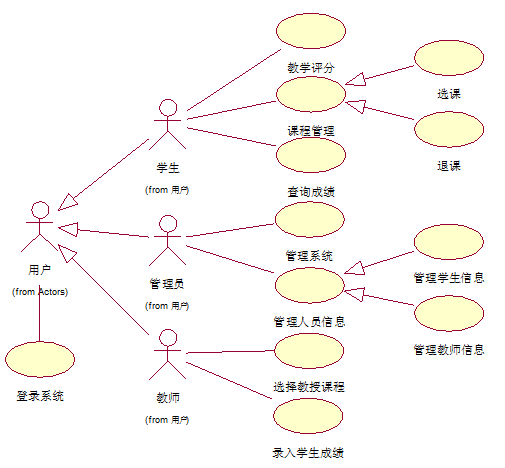
\includegraphics[width=\textwidth]{img/jwxt_usecases.png}
   \caption{教务系统用例析取图}
\end{figure}

\subsection{教务系统用例规约}
\subsubsection{选课用例的用例规约}

\begin{itemize}
  \item 简要说明
  
  \CJKindent 本用例允许学生注册本学期提供的课程。在学期开始的开放注册时期,学生可以添加或修改选择的课程。课程目录系统提供了当前学期开设的所有课程的列表。
  
  \item 事件流
  \begin{enumerate}
    \item 基本事件流
    
    用例开始于学生选择修改课程表,执行“添加课程”子事件流:
    \begin{enumerate}[(1)]
      \item 系统从课程目录系统中得到课程类别列表(公必、专必、公选、专选),并将列表显示给学生
      \item 学生选择课程类别
      \item 系统从课程目录系统中得到相应课程类别中的课程列表,对列表中的课程检验学生是否满足必要的前置条件,课程是否未被选满且没有时间冲突,然后将满足以上约束的课程列表显示给学生
      \item 学生从课程列表中选择课程
      \item 一旦学生决定了选择某门课程,系统将学生添加到该门课程,用该门课程的课程信息更新课程表,并用“已登记”在课程表中对该门课程进行标记
    \end{enumerate}

    \item 备选事件流
    \begin{enumerate}[{2}.1]
      \item 不满足前置条件,课程人数已满或课程时间冲突
      
      \CJKindent 如果在添加课程事件流中,系统确定学生没有满足必要的前置条件,或者选择的课程已满,或课程有时间冲突,将显示一条错误信息。学生可选择另一门课程,此用例继续;或取消操作,这时本用例重新开始。
      
      \item 未找到课程表
      
      \CJKindent 如果在增加或删除课程表子事件流中,系统无法返回学生的课程表,将显示错误消息。学生确认错误,这时本用例重新开始。
      
      \item 无法访问课程目录系统
      
      \CJKindent 如果系统无法与课程目录系统取得联系,系统将显示错误消息。学生确认错误,本用例终止。
      
      \item 课程注册系统被关闭
      
      \CJKindent 当用例开始时,如果确定用于本学期的注册系统已被关闭,显示一条消息给学生,本用例终止。学生不能在注册系统关闭后注册课程。
    \end{enumerate}
  \end{enumerate}
  
  \item 特殊需求
  
  \CJKindent 无
  
  \item 前置条件
  
  \CJKindent 本用例开始前学生必须已经登陆进系统,且注册员开放注册。
  
  \item 后置条件
  
  \CJKindent 如果用例成功,学生的课程表被创建,修改,删除。否则系统状态不变。
\end{itemize}

\begin{figure}[H]
  \centering
  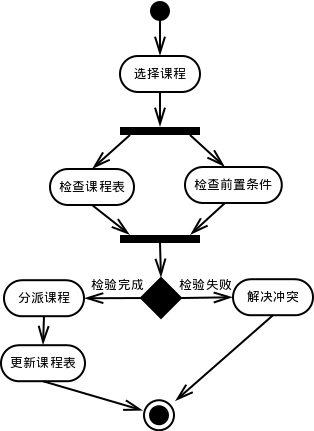
\includegraphics[scale=0.7]{img/jwxt_scourse.png}
  \caption{选课用例过程模型}
\end{figure}

\subsubsection{退课用例的用例规约}
\begin{itemize}
  \item 简要说明
  
  \CJKindent 本用例允许学生退选除本学期已选择的课程。从学期开始的开放注册时期到学期末的考试阶段前,学生可以退选本学期已选择的课程。
  
  \item 事件流
  \begin{enumerate}
    \item 基本事件流
    
    \CJKindent 用例开始于学生选择修改课程表,执行“删除课程”子事件流:
    \begin{enumerate}[(1)]
      \item 系统得到并显示学生当前的课程表
      \item 学生选择要删除的课程,必须选择的课程将不能被选择
      \item 系统检测待删除的课程是否满足必要的预备条件,是否未进入考试阶段,然后提示学生确认删除课程
      \item 学生确认删除
      \item 系统将学生从所选课程中删除,并更新课程表
    \end{enumerate}
    
    \item 备选事件流
    
    \begin{enumerate}[{2}.1]
      \item 不满足前置条件
      
      \CJKindent 如果在删除课程子事件流中,系统确定学生没有满足前置条件,将显示一条错误信息。学生可选择另一门课程进行删除,此用例继续;或取消操作,这时本用例重新开始。
      
      \item 未找到课程表
      
      \CJKindent 如果在删除课程子事件流中,系统无法返回学生的课程表,将显示错误消息。学生确认错误,这时本用例重新开始。

      \item 无法访问课程目录系统
      
      \CJKindent 如果系统无法与课程目录系统取得联系,系统将显示错误消息。学生确认错误,本用例终止。
      
      \item 选课阶段已结束
      
      \CJKindent 当用例开始时,如果确定本学期的选课阶段已结束,显示一条消息给学生,本用例终止。学生不能在选课阶段结束后退课。
    \end{enumerate}
  \end{enumerate}
  
  \item 特殊需求
  
  \CJKindent 无。
  
  \item 前置条件
  
  \CJKindent 本用例开始前学生必须已经登陆进系统,注册员开放注册,且考试阶段未开始。
  
  \item 后置条件
  
  \CJKindent 如果用例成功,学生的课程表被修改,否则系统状态不变。
\end{itemize}

\begin{figure}[H]
  \centering
  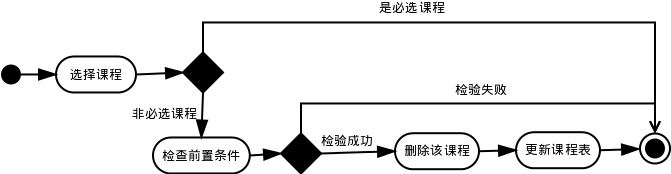
\includegraphics[scale=0.7]{img/jwxt_dcourse.png}
  \caption{退课用例过程模型}
\end{figure}

\subsubsection{教学评分用例的用例规约}

\begin{itemize}
  \item 简要说明
  
  \CJKindent 本用例允许学生对教师的教学进行教学评分。关闭注册后,学生可以对所选的任意一门课程进行教学评分,期间可以进行修改。在学生查看某一门课程的成绩前,必须先进行教学评分并确认对该门课程教师的教学所作的教学评分,此后教学评分不可修改。
  
  \item 事件流
  
  \begin{enumerate}
    \item 基本事件流
    
    \CJKindent 用例开始于学生选择教学评分。
    \begin{enumerate}
      \item 系统从课程表中得到学生所选课程,并将未标明“已评教”的课程信息列表显示给学生
      \item 学生从课程信息列表中选择要进行教学评分的课程
      \item 执行“进行教学评分”子事件流
    \end{enumerate}
    
    \begin{enumerate}[{1}.1]
      \item 进行教学评分
      \begin{enumerate}[(1)]
        \item 学生选择对该门课程所评的分数等级,同时可以在文本框中附加说明
        \item 一旦学生确认了教学评分,系统用当前课程的教学评分信息更新教学评分统计
        \item 执行提交教学评分子事件流
      \end{enumerate}
      
      \item 提交教学评分
      
      \CJKindent 系统用“已评教”在课程表中对该门课程进行标记。系统更新并保存课程表。
    \end{enumerate}
    
    \item 备选事件流
    \begin{enumerate}[{2}.1]
      \item 查看教学评分
      
      \CJKindent 学生选择要进行教学评分的课程后,可查看该门课程的历史教学评分信息,系统获取并显示当前课程新建以来累计的教学评分信息,包括选择各分数等级的人数及比例等。学生确认查看完历史教学评分信息后本用例继续进行。
      \item 未关闭注册
      
      \CJKindent 提示学生未关闭注册,需要在关闭注册后才能开始教学评分。
    \end{enumerate}
  \end{enumerate}
  
  \item 特殊需求
  
  \CJKindent 无
  
  \item 前置条件
  
  \CJKindent 注册员关闭注册。
  
  \item 后置条件
  
  \CJKindent 如果用例成功,任课老师教学评分信息被更改。否则系统状态不变。
\end{itemize}

\begin{figure}[H]
  \centering
  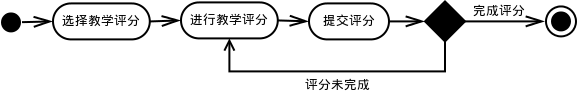
\includegraphics[scale=0.7]{img/jwxt_accessment.png}
  \caption{教学评分用例的过程模型}
\end{figure}

\subsubsection{查询成绩用例的用例规约}

\begin{itemize}
  \item 简要说明
  
  \CJKindent 本用例允许学生查询成绩。在查询成绩前,必须完成课程的教学评分,否则无法查询成绩。
  
  \item 事件流
  
  \begin{enumerate}
    \item 基本事件流
    
    \CJKindent 用例开始于学生查询成绩。
    \begin{enumerate}
      \item 系统检测学生是否完成教学评分,若已完成则显示学年度、学期、培养类别、课程类别、课程名称(可选)的选项,否则跳转到教学评分页面
      \item 学生选择相应查询选项
      \item 系统返回该学生相应课程的成绩并显示
    \end{enumerate}
    
    \item 备选事件流
    \begin{enumerate}
      \item 学生未完成教学评分
      
      \CJKindent 系统自动跳转到教学评分页面。
      
      \item 导出成绩
      
      \CJKindent 学生选择要导出的课程,系统将相应的课程成绩以xls格式导出并提供下载。
      
    \end{enumerate}
  \end{enumerate}
  
  \item 特殊需求
  
  \CJKindent 无。
  
  \item 前置条件
  
  \CJKindent 学生完成教学评分。
  
  \item 后置条件
  
  \CJKindent 无
\end{itemize}

\begin{figure}[H]
  \centering
  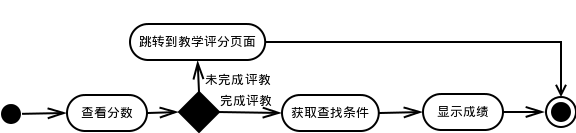
\includegraphics[scale=0.7]{img/jwxt_viewscore.png}
  \caption{查看分数用例的过程模型}
\end{figure}

\subsection{教务系统补充规约}

\begin{enumerate}
  \item 目标
  
  \CJKindent 本文档的目的是定义教务系统的需求。本补充规约列出了不便于在用例模型的用例中获取的系统需求。补充规约和用例模型一起记录关于系统的一整套需求。
  
  \item 范围
  
  \begin{enumerate}
    \item 本补充规约适用于教务系统,将要由学习面向对象软件分析与设计的学生开发。
    \item 本规约除定义了在许多用例中共有的功能性需求以外,还定义了系统的非功能性需求,例如:可靠性、可用性、性能和可支持性等。(功能性需求在用例规约中定义。)
  \end{enumerate}
  
  \item 参考
  
  无。
  
  \item 功能
  
  \begin{enumerate}
    \item 多个用户必须能同时执行操作。
    \item 如果某个学生所建的课程表中包含人数已满的课程,必须通知这位学生。
  \end{enumerate}
  
  \item 可行性
  
  \CJKindent 用户界面应与IE7/8/9/10、Chrome、Firefox、Safari等主流浏览器兼容。
  
  \item 可靠性
  
  \CJKindent 教务系统在每周七天,每天二十四小时内都应是可以使用的。宕机的时间应少于10\%。
  
  \item 性能
  
  \begin{enumerate}
    \item 在任意既定时刻,系统最多可支持2000名用户同时使用中央数据库,并在任意时刻最多可支持500名用户同时使用本地服务器。
    \item 系统将能在十秒钟内提供对课程目录系统数据库的访问。
    \item 注意:基于风险的原型发现课程目录系统数据库在没有利用中层处理能力的前提下,无法满足性能上的需求。
    \item 系统必须能够在2分钟内完成所有事务的80\%。
  \end{enumerate}
  
  \item 可支持性
  
  \CJKindent 无。
  
  \item 安全性
  
  \begin{enumerate}
    \item 系统必须能防止学生修改他人的课程表以及教师修改其他教师所开设的课程。
    \item 只有一门课的教师能输入学生该门课的成绩。
    \item 只有注册员能更改学生的信息。
  \end{enumerate}
  
  \item 设计约束
  
  \begin{enumerate}
    \item 该系统应与现有课程目录系统(是RDBMS数据库)集成在一起
    \item 系统必须提供可用于各大主流浏览器(IE、Chrome、Safari、Firefox等)的用户接口
  \end{enumerate}
\end{enumerate}

\subsection{术语表}
  \begin{table}[H]
    \caption{术语表}
    \begin{tabularx}{\textwidth}{|l|l|X|l|}
    \hline
    \textbf{术语} & \textbf{英语名称} & \textbf{定义和信息} & \textbf{别名}\\
    \hline
    课程&Course&学生所需学习的科目及其安排&\\
    \hline
    课程表&Schedule&学生所选课程的列表及其详细信息&\\
    \hline
    课程成绩&Achievement&日常考核、期末考试分数、排名等评定的数值&\\
    \hline
    考核方式&Examining Method&考试的形式,包括提交报告、开卷考试、闭卷考试等&\\
    \hline
    课容量&Capacity&课程可以容纳的学生人数&\\
    \hline
    课程类别&Course Type&课程的分类,包括公共必修课、公共选修课、专业必修课与专业选修课&\\
    \hline
    培养类别&Category&包括主修、辅修、双专业和双学位&\\
    \hline
    教学评分&Assessment&对教师进行教学评价&评教\\
    \hline
    开课计划&Course Arrangement&课程开设的安排与进度&\\
    \hline
    学籍信息&Student Information&包含学生的个人信息、学习经历&\\
    \hline
    注册&Registration&学生选择课程或老师添加课程信息&\\
    \hline
    退选&Withdrawal&学生取消选择课程&\\
    \hline
    查询成绩&Query Achievement&显示学生的课程成绩、排名、平均绩点&\\
    \hline
    B/S结构&Browser/Server Architecture&Browser/Server 浏览器/服务器结构&\\
    \hline
  \end{tabularx}
  
\end{table}


\subsection{测试用例设计}
\begin{enumerate}
  \item 添加课程
  \begin{itemize}
    \item 前置条件:学生用户选择添加课程选项。
    \item 设计:
    \item 步骤——系统从课程目录系统中得到可选择的课程列表,并将列表显示给学生。
    \item 检验点——课程列表正确地被显示。
    \item 步骤——显示空白课程表并提示学生选择四门主要课程和两门备选课程;
    \item 检验点——空白课程表被正确地显示。
    \item 步骤——如果学生选择相应课程并提交。
    \item 检验点——如果课程选择符合条件,则所选课程标记为已登记。
    \item 检验点——系统正确地保存了课程表。
    \item 检验点——在课程人数已满,有时间冲突,课程数量不符的异常情况下,系统是否做出预期的反应。
    \item 步骤——如果学生选择相应课程并保存。
    \item 检验点——所选课程标记为已选。
    \item 检验点——系统正确地保存了课程表。
    \item 后置条件:成功测试该用例后,确保退出注册课程。
    \item 可接受标准:所有的检验点必须成功。
  \end{itemize}
\end{enumerate}
